\subsection{Qt Creator}

\begin{frame}
  \frametitle{Qt Creator\footnote
    {\url{https://www.qt.io/ide/}} \footnote{\url{http://doc.qt.io/qtcreator/}}}
  \small
  \begin{itemize}
    \item Cross-platform IDE / rapid development tool for Qt-based applications.
    \begin{itemize}
      \item Code editor with code-completion and syntax highlighting.
      \item Project and resource management
      \item Build system integration (\texttt{qmake}, \texttt{moc}, \texttt{rcc},
        \texttt{uic}, etc.)
      \item Debugger
      \item Visual form designer for both widget-based and \texttt{qml}-based
        applications.
      \item Tool for easy internationalization and translation of texts to
        other languages.
      \item Integration with popular version control systems like git, mercurial,
        subversion and others.
      \item Configurable keyboard shortcuts.
    \end{itemize}
  \end{itemize}
\end{frame}

\begin{frame}
  \frametitle{Qt Creator -- code editor}
    \begin{figure}[!t]
    \centering
    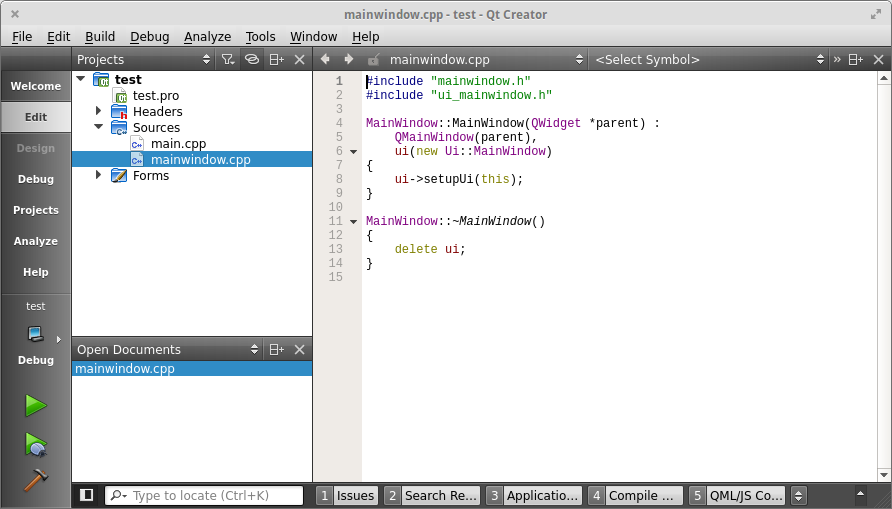
\includegraphics[width=\textwidth]{images/qt_creator1.png}
    \end{figure}
\end{frame}

\begin{frame}
  \frametitle{Qt Creator -- form designer}
    \begin{figure}[!t]
    \centering
    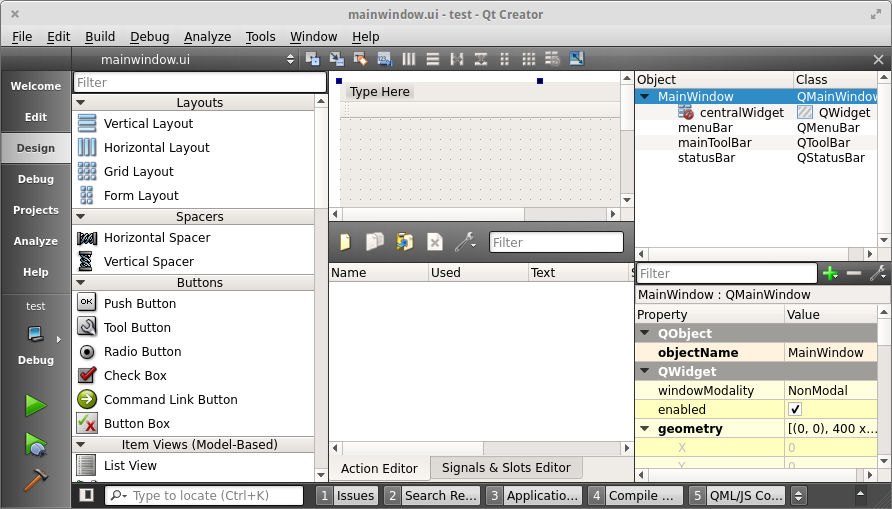
\includegraphics[width=\textwidth]{images/qt_creator2.png}
    \end{figure}
\end{frame}

\begin{frame}
  \frametitle{Qt Creator -- default shortcuts for common actions\footnote
     {\url{http://doc.qt.io/qtcreator/creator-keyboard-shortcuts.html}}}
     \tiny
     \begin{columns}
       \begin{column}{0.5\textwidth}
       \rowcolors{2}{green!80!yellow!50}{green!70!yellow!40}
       \begin{tabular}{|p{0.65\textwidth}|p{0.25\textwidth}|}
         \hline
         \textbf{Action} & \textbf{Shortcut} \\
         Activate locator & Ctrl+K \\
         \hline
         Switch to Welcome mode & Ctrl+1 \\
         \hline
         Switch to Edit mode & Ctrl+2 \\
         \hline
         Switch to Design mode & Ctrl+3 \\
         \hline
         Switch to Debug mode & Ctrl+4 \\
         \hline
         Switch to Projects mode &Ctrl+5 \\
         \hline
         Switch to Analyze mode & Ctrl+6 \\
         \hline
         Switch to Help mode & Ctrl+7 \\
         \hline
         Toggle the sidebar & Alt+0 \\
         \hline
         Toggle Issues pane & Alt+1 \\
         \hline
         Toggle Search Results pane & Alt+2 \\
         \hline
         Toggle Application Output pane & Alt+3 \\
         \hline
         Toggle Compile Output pane & Alt+4 \\
         \hline
         Toggle other output panes & Alt+number \\
         \hline
         Activate Bookmarks pane & Alt+M \\
         \hline
         Activate File System pane & Alt+Y \\
         \hline
         Activate Open Documents pane & Alt+O \\
         \hline
         Activate Projects pane & Alt+X \\
         \hline
         Full screen & Ctrl+Shift+F11 \\
         \hline
       \end{tabular}
       \end{column}
       \begin{column}{0.5\textwidth}
       \rowcolors{2}{green!80!yellow!50}{green!70!yellow!40}
       \begin{tabular}{|p{0.65\textwidth}|p{0.25\textwidth}|}
         \hline
         \textbf{Action} & \textbf{Shortcut} \\
         \hline
         Open file or project & Ctrl+O \\
         \hline
         New file or project & Ctrl+N \\
         \hline
         Select all & Ctrl+A \\
         \hline
         Delete & Del \\
         \hline
         Cut & Ctrl+X \\
         \hline
         Cut line & Shift+Del \\
         \hline
         Copy & Ctrl+C \\
         \hline
         Copy line & Ctrl+Ins \\
         \hline
         Paste & Ctrl+V \\
         \hline
         Undo & Ctrl+Z \\
         \hline
         Redo & Ctrl+Y \\
         \hline
         Print & Ctrl+P \\
         \hline
         Save & Ctrl+S \\
         \hline
         Save all & Ctrl+Shift+S \\
         \hline
         Quit & Ctrl+Q \\
         \hline
         Close window & Ctrl+W \\
         \hline
         Close all & Ctrl+Shift+W \\
         \hline
         Close current file & Ctrl+F4 \\
         \hline
         Trigger a completion in this scope & Ctrl+Space \\
         \hline
       \end{tabular}
       \end{column}
     \end{columns}
\end{frame}

